\makechapter{A Binary Theory of Collapse}{A Binary Theory of Collapse}{Jacob Gong}{Silicon Valley High School}{10.17613/z9x7w-wky93}

To begin our inquiry into the nature of civilizational collapse, a definition of relevant terms is obligatory. 

For the purposes of this essay, “civilizational collapse” shall be defined as a substantial decrease of human populations, and/or of political, scientific, or cultural complexity in some local area (\cite[p.\ 363]{diamond1994ecological}). Here, decreasing complexity is defined as the abandoning of advanced technology, economic regression, simplification of social bonds, loss of territory, increased decentralization, reduced trade, and/or curtailed information exchange (\cites[chap.\ 1]{tainter1988collapse}{tainter2023lecture}).

In this essay, I contend that civilizations collapse due to anthropological factors, environmental factors, and anthropogenic climate change (ACC), otherwise known as “global warming”. Moreover, I argue that our civilization will collapse since anthropogenic factors are immutable, environmental factors are unreliable and unpreventable, and ACC exhibits both properties. 

\section{Binary Theory of Collapse}

The binary theory of collapse (BTC) comprises two major constituents (see fig.\ 1): anthropological and environmental. The anthropological factors are further divided into two components, what I will term the collective and individual factors, the former stems from biological necessity (\cite[p.\ 13]{santos2015evolutionary}), and the latter from genetic circumstance (\cites[p.\ 8]{goriounova2019genes}[pp.\ 1–3]{wu2020genetic}). Environmental factors are of two causally connected elements: natural disasters and natural climate fluctuations (NCFs). The former can cause the latter, or, in rarer instances, be civilization-ending in and of itself. ACC, a uniquely modern product, will be discussed in section IV. 

\subsection{Anthropological Factors}

The anthropological factors are divided into two strands: collective and individual. Collective factors have the property of being universally applicable, while individual factors are restricted to, as the name would suggest, individuals. There are two basic types of collective factors: \emph{sustentative-reproductive} and \emph{myopic.}

Sustentative-reproductive factors are ones directed towards the maintenance and nourishment of human beings and the biological want to reproduce. Examples of this include food production, construction, and manufacturing of health-related products, all of which are crucial for reproduction. However, we effectuate unintended destruction of the natural environment, overhunting, overfishing, soil depletion, salinization, erosion, and so forth (\cite{diamond2017youtube}). This leads to a Malthusian population crisis, where population rises above the productive output of a civilization. 

Myopic factors refer to “present bias” within the human decision-making process, i.e., we tend to prefer smaller rewards now, than larger rewards later (\cite[p.\ 1]{chakraborty2021present}). Evolutionarily, uncertainty regarding future rewards have adapted our brain to prioritize immediate gratification over delayed gratification (\cite[p.\ 1]{albrecht2013what}). Myopic factors are especially prominent in societies with high Gini ratios. In such societies, the powerful are potentially unaffected by actions whence they benefit, while the lower classes suffer the brunt of the negative ramifications (\cite{paulson2015shorttermism}). For instance, while oil barons would certainly support fracking practices, the environmental consequences have the greatest effect for the impoverished (\cite{lin2022fracking}).

Individual factors are similarly most applicable for individuals wielding power. There are two categories of individual factors: egoistic and irrational. Historic examples of individual factors are scarce when compared with evidence for the other factors, though this is not because they are less common. In many circumstances, records are scant or even non-existent, simply due to the great magnitude of time which has passed since the collapse of said civilization. Another possibility is that of revisionist historiography fueled by some ideological values, perhaps some concerted attempt at removing a figure from the historical record (\cite{burton2020akhenaten}). 

Egoistic factors pertain to selfishness and indifference to the plight of others. Selfishness, when combined with substantial amounts of power, can lead to unwarranted risk taking, abuse of subordinates, aggression, and duplicity, all of which produces instability and volatility (\cites{simmons2024narcissistic}[pp.\ 9–10]{blanton2020moral}). 

Irrational factors denote acting seemingly without reason and foresight. Often, this may simply be the result of misinformation, inexperience, or misfortune, not necessarily an inherent illogicality. Collapse caused by irrational factors can be likened to the Red Queen Hypothesis, in that such collapse would be irregular and erratic (\cite{kemp2019collapse}). 

\subsection{Environmental Factors}

Environmental factors are twofold: natural disasters and natural climate fluctuations. 

Natural disasters have been recorded, though only on rare occasions, to be the direct cause of civilizational collapse. There have been examples of invasive diseases, immense floods and volcanic eruptions leading to the destruction of civilization (\cites[p.\ 289]{ehrenpreis2022historical}[p.\ 1]{rincon2014doggerland}). Nonetheless, it should be noted that natural disasters typically only have a small area of effect, which nullifies it ability to directly injure large civilizations. 

More frequently, however, it is the NCFs caused by some natural disaster which carries the most potent destructive power. For example, a declining, plague-stricken population could cause reforestation due to their impaired ability to engage in logging. Accordingly, the natural carbon sink grows, reducing the global temperature, leading to crop failures (\cites[p.\ 9]{nevle2011neotropical}{juurakko2021cold}). 

NCFs could also occur independently, such as through El Niño and La Niña, altered ocean currents, Milankovitch cycles, or changes in solar activity (\cites[p.\ 1]{loury2016drought}[p.\ 6]{berger2006equatorial}[pp.\ 5–6]{lockwood2010cold}). These have been recorded to produce adverse effects in civilizations (\cite[p.\ 292]{columbia2010angkor}).

\section{Examples}

The collapse of Pacific Island societies provides a striking illustration of the impacts of the substantive-reproductive factors. The Māori peoples, who, around the 14th century, settled New Zealand, hunted many native species to extinction, including the Moa and the New Zealand swan (\cites[p.\ 358]{walter2017polynesian}[p.\ 4922]{allentoft2014extinct}[p.\ 1]{rawlence2017blackswans}). They also extensively reduced the population of species such as fur seals and sea lions (\cite[p.\ 1]{wilmshurst2007deforestation}). These factors, combined further with comprehensive deforestation, caused a drastic decline in the local population. Similar trends were observed in other locations, including the Mangareva, Henderson, and Kaho‘olawe Islands (\cites[p.\ 5]{fagan2010great}[p.\ 132]{diamond2005collapse}[p.\ 443]{rolett2004deforestation}[p.\ 336]{diamond1994ecological}). Additionally, myopic and anthropogenic factors could have been at play. However, due to the lack of information regarding the pre-European history of the Polynesian islands, this is difficult to ascertain.  

From the Late Bronze Age Collapse, we can find numerous examples showcasing the impact of natural disasters on the environment. The Hekla 3 eruption, occurring around the 12th century BCE, caused famines and compounded preexisting droughts (\cites[p.\ 340]{baker1995hekla}[pp.\ 456–458]{yurko1999end}[p.\ 719]{manning2023hittite}). Consequently, human immune systems were weakened, and bubonic plague became widespread (\cite[p.\ 1]{spyrou2018plague}). The Sea Peoples, often cited as the primary cause for the Late Bronze Age Collapse, began their exodus to the major Mediterranean civilizations, driven by droughts of their own (\cite[pp.\ 16–17]{carpenter1966discontinuity}). All the aforementioned factors, combined with the increasing wealth gap of the Late Bronze Age, led to the downfall of those once mighty pillars of civilization (\cites[pp.\ 20–22]{basri2020wealth}{weisweiler2022inequality}). 

The Byzantine historian Procopius describes egoistic factors at play in the collapse of the Western Roman Empire. As he describes, when emperor Honorius was informed of the sack of Rome in 410 CE, he cried, “And yet it has just eaten from my hands!”, referring to his favorite pet chicken, coincidentally named Roma. When it was explained that the city had fallen, and not his pet chicken, Honorius supposedly sighed with relief (\cite{procopius1916vandalic}). Though the story is widely believed to be apocryphal, it aptly demonstrates the incompetence and self-absorption of the ruling elite (\cite[p.\ 643]{gibbon1845decline}). Many of the final Western Roman Emperors in the 5th century shared in these qualities (\cite{britannica2024majorian}). Environmental factors likewise contributed greatly to the fall of the empire. In the third century, the Northwestern provinces saw climate fluctuations; a century later, severe droughts forced the Huns to migrate into Roman territory and ultimately weakened Rome. (\cite[pp.\ 190–191]{mccormick2012climate}). Extensive deforestation for arable land and air pollution from incinerated lumber was also recorded (\cites[p.\ 173]{harris2013ancient}[p.\ 171]{erskine2012companion}). Once again, we find that wealth inequality can be observed, as records show that ~1.4\% of the population controlled around 16-29\% of the total wealth (\cite[p.\ 76]{scheidel2009size}).

For another example of individual factors at play in civilizational collapse, we can turn to the Mughal Empire. Akbar the Great, the founder of the empire, promoted a policy of religious toleration, in the process improving the governing bureaucracy and ensuring stability (\cites{ballhatchet2024akbar}[p.\ 159]{stein2010historyindia}). However, though the system was carefully maintained by the next two emperors, emperor Aurangzeb, the third after Akbar, increasingly favored Muslims in his rulings, abandoning the policy of toleration (\cite[p.\ 183]{pletcher2010historyindia}). Thus, the Mughal empire became progressively more fractured and debilitated until it was finally subsumed by the British East India Company in the mid-18th century (\cites[p.\ 8]{blanton2020moral}{nationaltrust2024eastindia}). 

\section{Our Collapse}

Based on the metrics proposed in the BTC, it is more than likely that human civilization will collapse. Let us analyze each factor of the BTC individually and delineate the way in which they are applicable today: 

First, the sustentative-reproductive factor; namely, the conjoined problems of overpopulation and food scarcity. Currently, 10\% of the world faces chronic hunger (\cite{omer2024hunger}). By 2050, we would need to double our current agricultural output in order to meet consumption demands (\cite{ranganathan2018feed10billion}). However, in attempting to increase agricultural output, we would cause the toxification and pollution of the environment (\cite[p.\ 3]{chowdhury2022agricultural}). Yet, said pollution cyclically contributes to the stunting of crop yields (\cite{jordan2022pollution}). This may result in a positive feedback loop, resulting in both further environmental degradation and instances of persistent hunger and famine. 

Second, myopic factors, which can be seen in many of the world governments and international organizations today. For instance, despite progress made against overconsumption by American President Jimmy Carter in the late 1970s, the Reagan administration reversed this trend in support of their ideological values and to curry favor with the oil industry (\cite{mckibben2021they}). More recently, despite the optimistic objectives set during the 2015 Paris Agreement, none of the top four emitters – the United States, China, the EU, and India – have met their emission reduction targets (\cite{bearak2022world}). 

Third, individual factors, which can be difficult to identify in the short-term. However, this factor can be found in the conducts of American President Donald Trump, who has taken an ambiguous stance towards ACC despite clear evidence of its existence (\cite{cheung2020trump}). Furthermore, Trump’s Affordable Clean Energy policy, which supplanted the Clean Power Plan, increased emissions despite aiming to do the opposite (\cite[p.\ 9]{keyes2019ace}). 

Fourth, NCFs. Although mostly overshadowed by ACC, NCFs still play a key role in global climate variation (\cite{shaftel2023vitalsigns}). Climate patterns such as El Niño and La Niña will continue to impact precipitation and temperature in the Americas and other parts of the world (\cite{halpert2014elnino}). Additionally, solar output levels and Milankovitch cycles will remain, albeit to a minimal degree, a consideration in climate trends (\cites{nasa2019sunrole}{nasa2020milankovitch}). 

Lastly, we must contend with the greatest existential menace facing humanity today: ACC (\cite{un2021biggestthreat}). Occupying the divide between the anthropological and environmental factors, ACC is the most concrete and substantial of the previously considered factors of collapse in our modern day. While originating with human activity, ACC impacts us in ways more akin to environmental factors (\cite[p.\ 896]{ipcc2014physical}). 

Beginning with the industrial revolution, global temperature has risen by around 1.1 \textsuperscript{o}C or 2 \textsuperscript{o}F (see fig.\ 2), which, despite seemingly being insignificant, has momentous consequences for the future of civilizations (\cite{lindsey2024globaltemp}). The increased temperature leads to more frequent wildfires, increased destructiveness and regularity of storms, higher frequency of drought, rising sea levels, magnified health risks, etc (\cites[p.\ 1]{diffenbaugh2021wildfire}[p.\ 4]{aumann2008frequency}[pp.\ 14–16]{dai2011drought}[p.\ 1]{meehl2005howmuch}[p.\ 5]{vermeer2009sealevel}{epa2022airquality}). 

These factors, all interconnected and reciprocally collaborating, can contribute to civilizational collapse, as demonstrated by figure 3 (\cite[p.\ 7]{kanter2009warming}). When compared with past climate events, ACC is of a much greater magnitude (\cite{nasa2010globalwarming}). Despite modern scientific advancements in reducing emissions and green energy, global temperatures are expected to continue to rise well into the future (\cite{ucar2021predictions}). Taking into account the effect climate change events have had on human civilizations hitherto, the future seems bleak (\cite[pp.\ 190–191]{natgeo2007visual}).

Lastly, with the advent of globalization, the collapse of one civilization could spread to other nations at an alarming rate. If a pandemic on the scale of the 1917 Spanish Flu were to occur in the modern day, it would kill nearly 33 million people in just the first six months (\cite{gates2018shattuck}). We can reasonably conclude that the magnitude of civilizational collapses in the contemporary era would surpass all previous collapses witnessed in the Anthropocene (\cite{juling2023future}). 

\section{Conclusion}

Supported by the aforementioned factors, I thus assert that civilizations collapse due to anthropological factors, environmental factors, and, more recently, ACC. In addition, as the evidence compiled in section IV would suggest, I contend that our civilization will collapse. 

\newpage

\section{Appendix}

\begin{figure}[h]
\centering
\begin{tikzpicture}[
    venn/.style={draw, thick, circle, minimum width=9cm},
    lab/.style={font=\large},
    txt/.style={align=left}
]
% Circle centers
\coordinate (L) at (0,0);
\coordinate (R) at (5.2,0); % adjust for overlap

% Circles
\node[venn] (A) at (L) {};
\node[venn] (E) at (R) {};

% Top labels
\node[lab, above=2mm of A.north] {Anthropological};
\node[lab, above=2mm of E.north] {Environmental};

% Left-circle bullet lists
\node[txt, anchor=west] at ($(A.center)+(-2.8,1.3)$) {\textbf{Collective:}};
\node[txt, anchor=west] at ($(A.center)+(-2.8,0.5)$) {$\bullet$ \; Sustentative\\\quad--reproductive};
\node[txt, anchor=west] at ($(A.center)+(-2.8,-0.3)$) {$\bullet$ \; Myopic};

\node[txt, anchor=west] at ($(A.center)+(-2.8,-1.0)$) {\textbf{Individual:}};
\node[txt, anchor=west] at ($(A.center)+(-2.8,-1.7)$) {$\bullet$ \; Egoistic};
\node[txt, anchor=west] at ($(A.center)+(-2.8,-2.3)$) {$\bullet$ \; Irrational};

% Intersection label
\node[txt] at ($(L)!0.5!(R)$) {\parbox{3.2cm}\centering
Anthropogenic\\[2pt] Climate Change};

% Right-circle text
\node[txt] (ND) at ($(R)+(2,2.2)$) {\parbox{3.6cm}\centering Natural\\ Disasters};
\node[txt] (NCF) at ($(R)+(2,-1.6)$) {\parbox{3.6cm}\centering Natural\\ Climate\\ Fluctuations};

% Dashed arrow with label
\draw[dashed, -stealth] (ND.south) -- (NCF.north);
\node[txt, rotate=90] at ($(ND.south)!0.5!(NCF.north)+(-0.7,0)$) {Potentially\\ causes};

\end{tikzpicture}
\caption{Venn diagram representing the binary theory of collapse. (Chart by author)}
\end{figure}

\newpage

\begin{figure}[h]
\centering
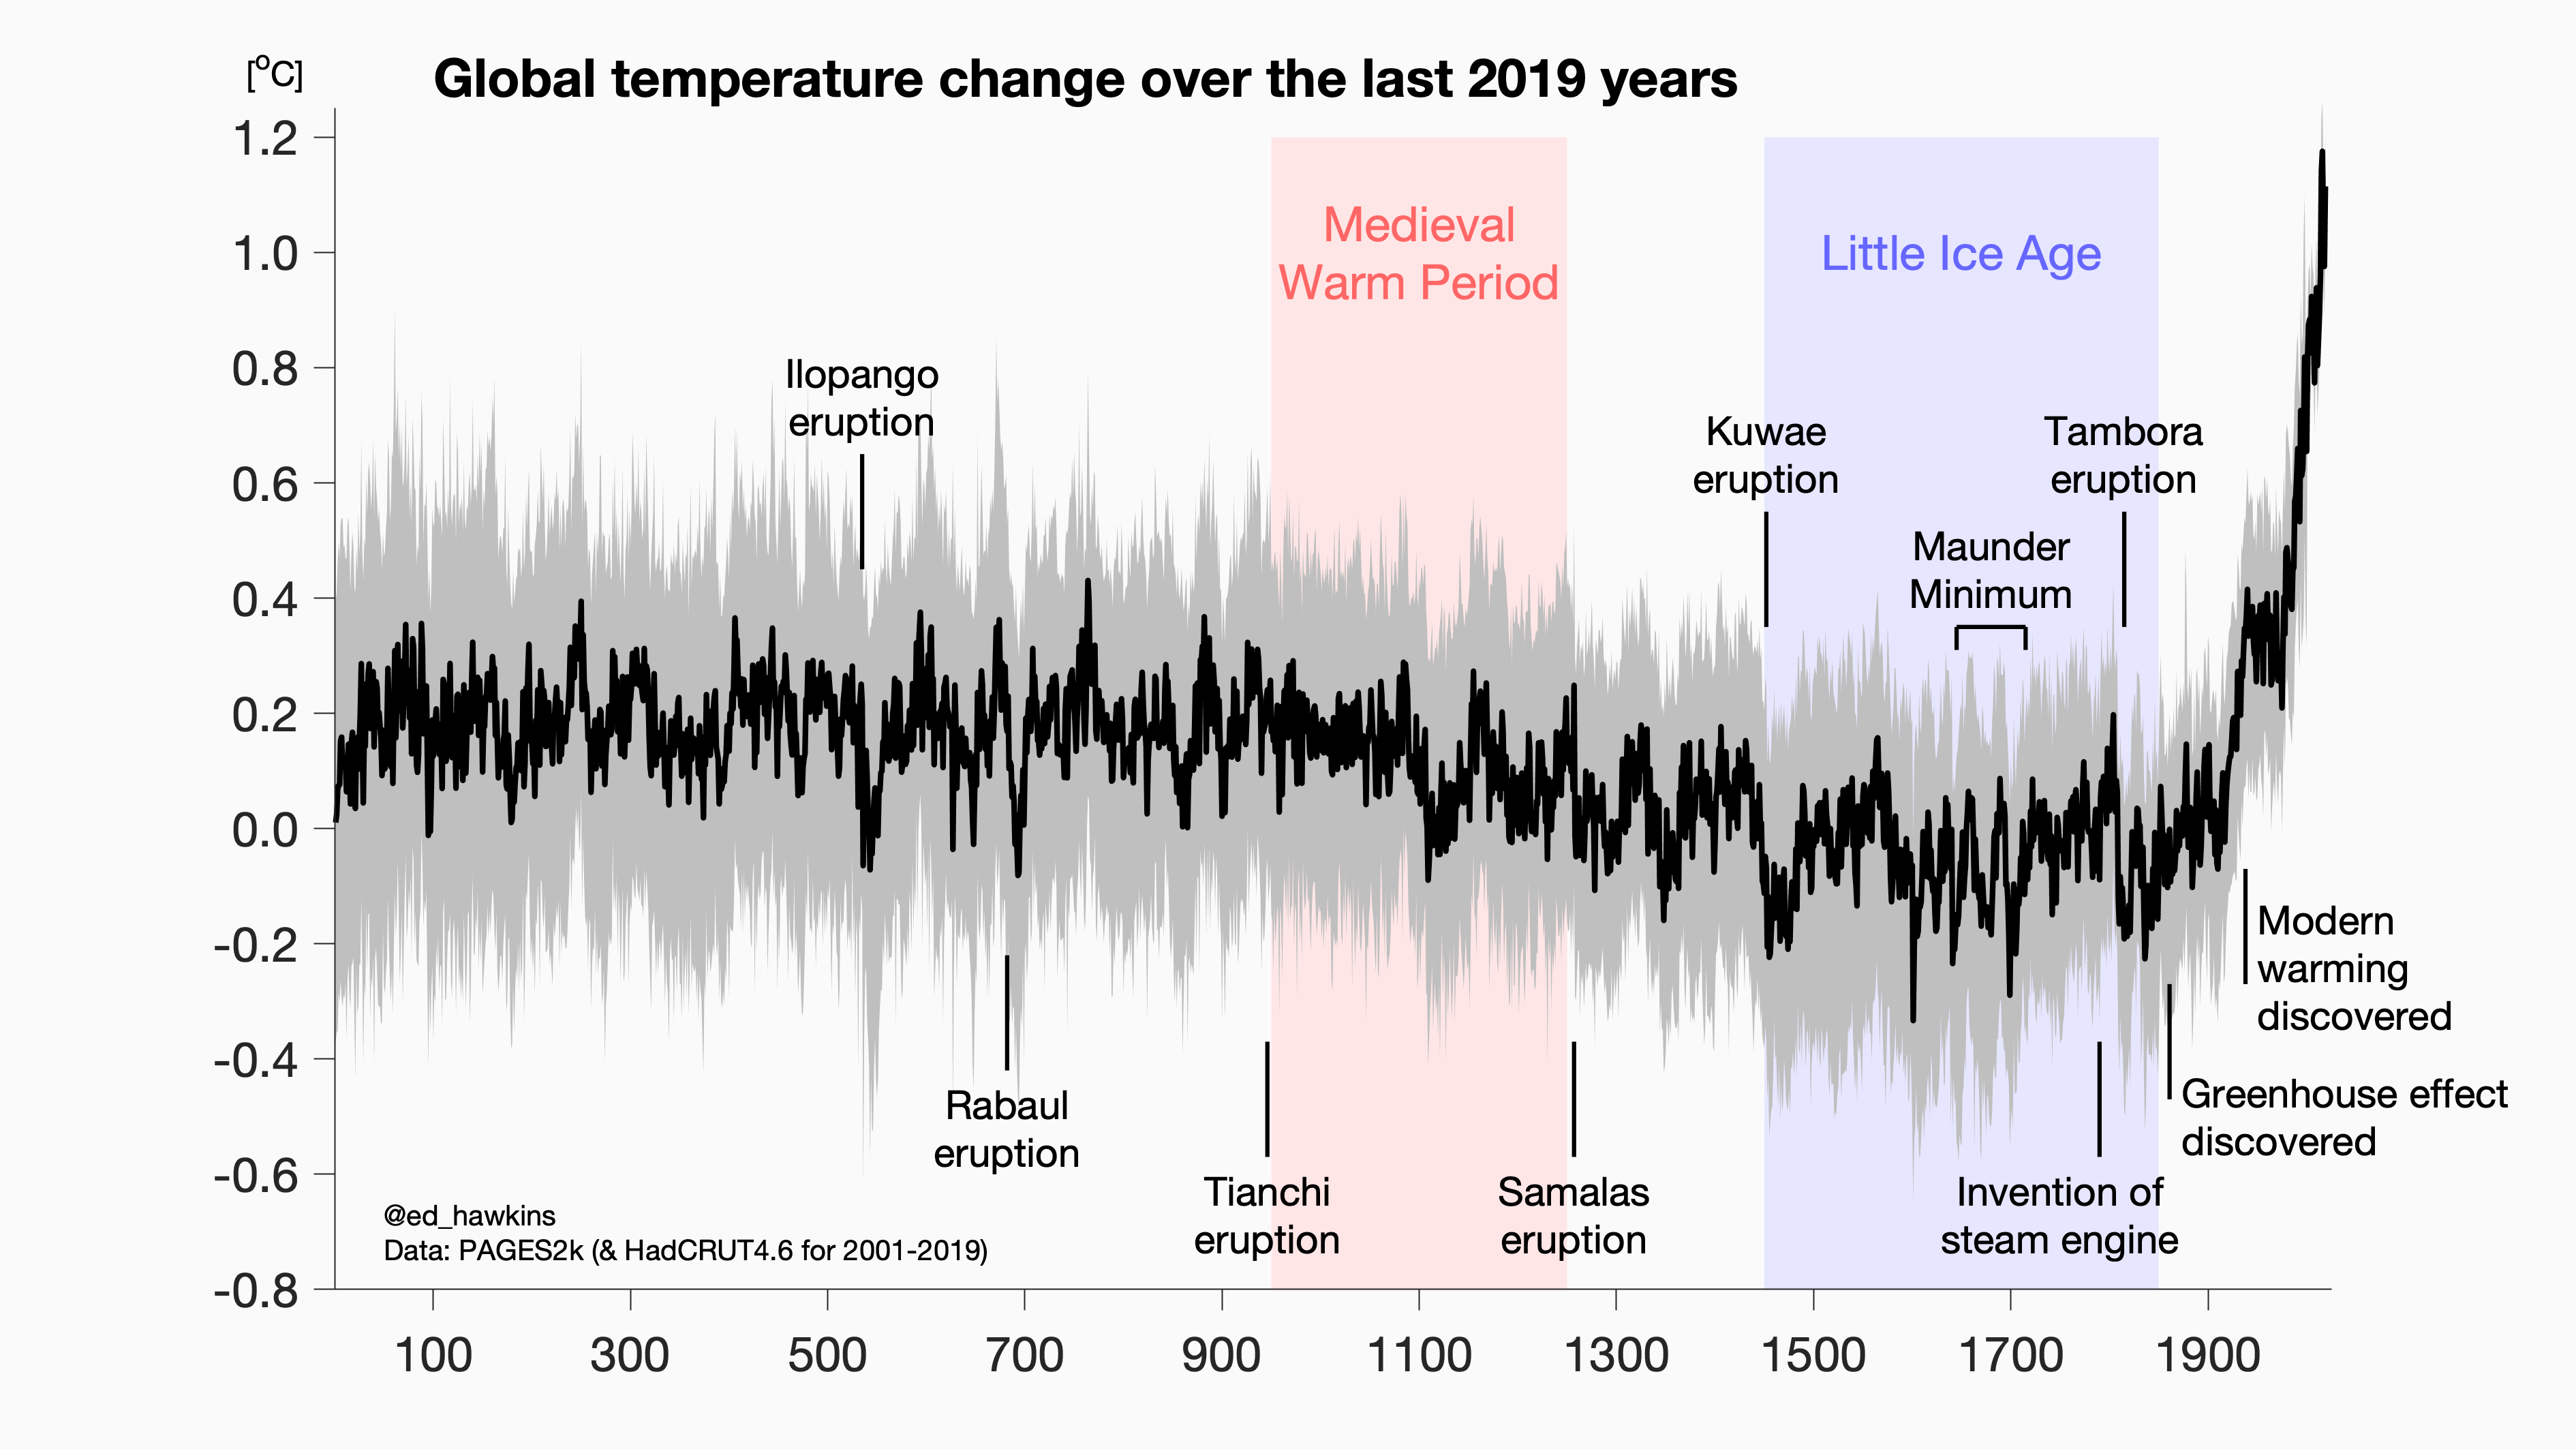
\includegraphics[width=0.9\linewidth]{lia_mwp-1.png}
\caption{The change in global temperature since 0 AD, Chart ``Global temperature change over the last 2019 years,'' from Ed Hawkin, \emph{2019 years.}}
\end{figure}

\newpage

\begin{figure}[h]
\centering
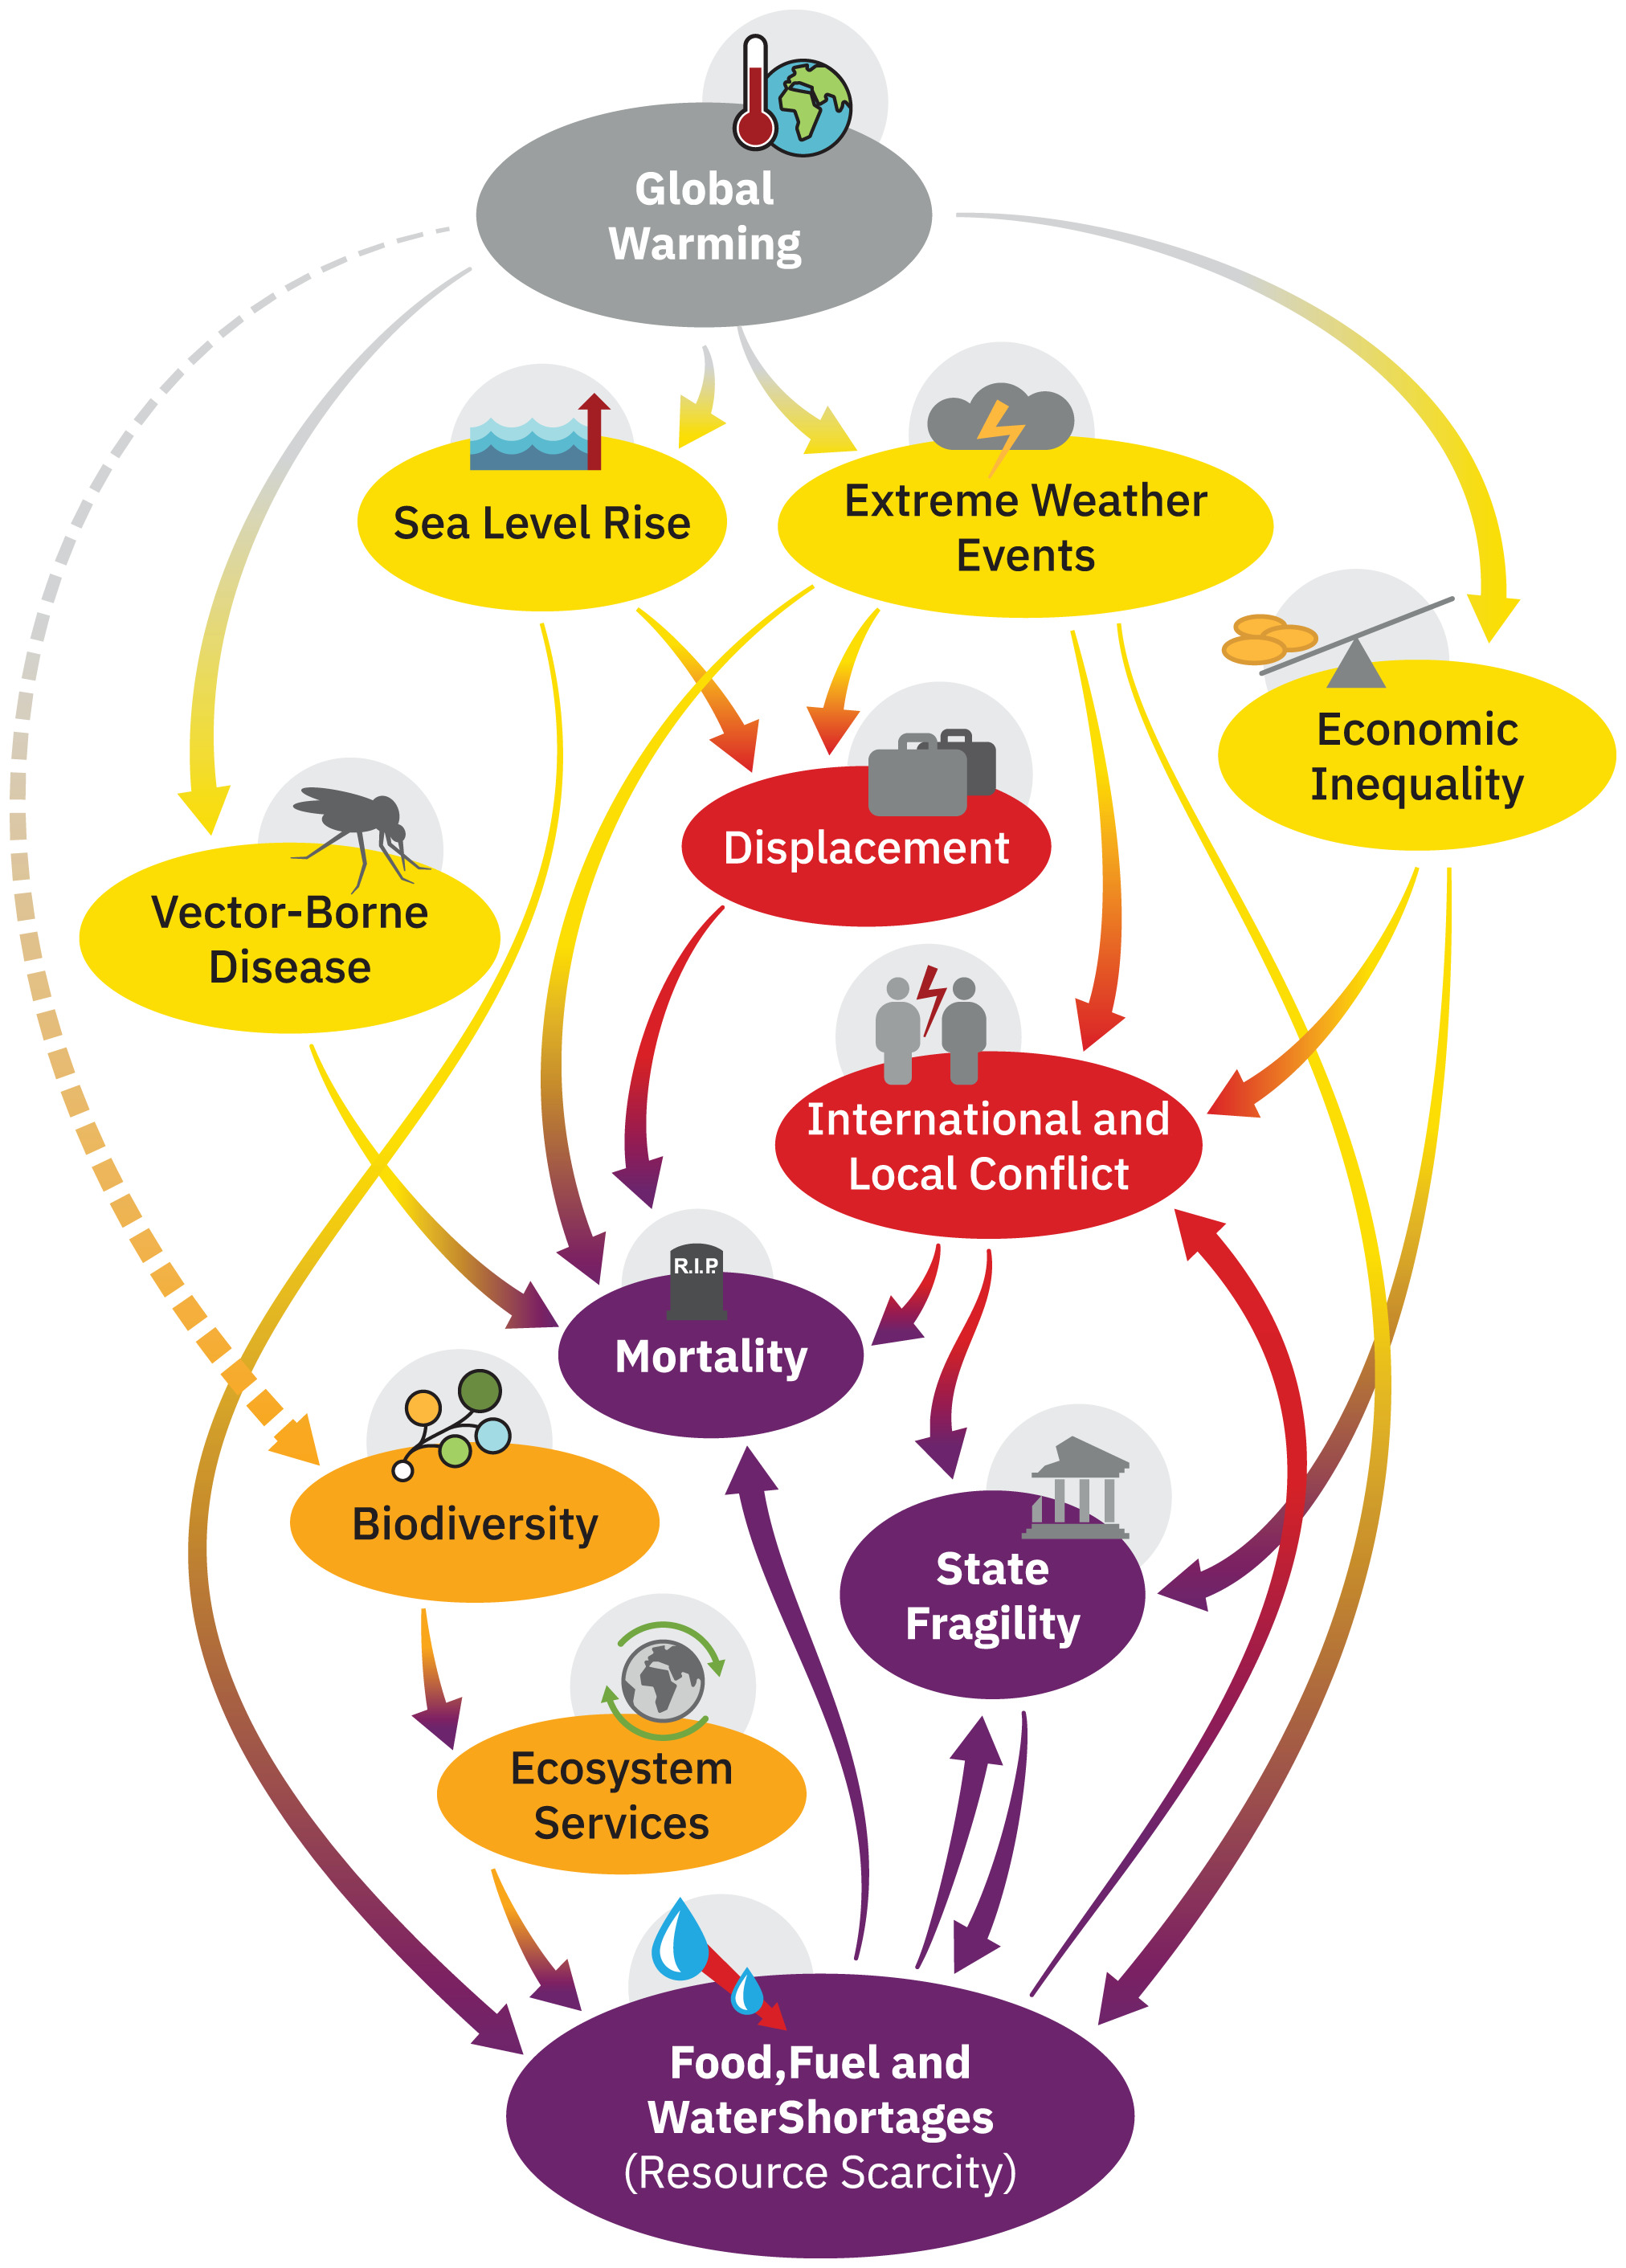
\includegraphics[width=0.6\linewidth]{pnas.2108146119fig03.jpg}
\caption{Causal loop diagram illustrating global climate failure, Chart, “Cascading global climate failure,” from Kemp et al., “Climate Endgame: Exploring catastrophic climate change scenarios”, PNAS, 119, no.34 (2022), fig. 3, \url{https://doi.org/10.1073/pnas.2108146119}}
\end{figure}

\newpage